\documentclass[a4paper]{article}

\usepackage[english]{babel}
\usepackage[utf8]{inputenc}
\usepackage{fullpage}
\usepackage{amsmath}
\usepackage{graphicx}
\usepackage[colorinlistoftodos]{todonotes}
\usepackage{hyperref}
\usepackage{amssymb}
\usepackage{outline} \usepackage{pmgraph} \usepackage[normalem]{ulem}
\usepackage{graphicx} \usepackage{verbatim}
% \usepackage{minted} % need `-shell-escape' argument for local compile

\usepackage[UTF8]{ctex}
\usepackage[inkscapeformat=png]{svg}

\title{
    \vspace*{1.0in}
    \includesvg[width=2.75in]{figures/logo.svg} \\
    \vspace*{1in}
    \textbf{\Huge Biweekly Report}
    \vspace{0.5in}
}

\author{ \\
    \textbf{\huge userElaina} \\
    \vspace*{1in}
}

\date{\LARGE 八月下}
\setcounter{page}{-1}
\newpage

\begin{document}
\LARGE

\maketitle
\tableofcontents
% \setcounter{page}{0}
\thispagestyle{empty}
\newpage

\section{RNN 的 BPTT 算法}

\begin{figure}[hb]
    \centering
    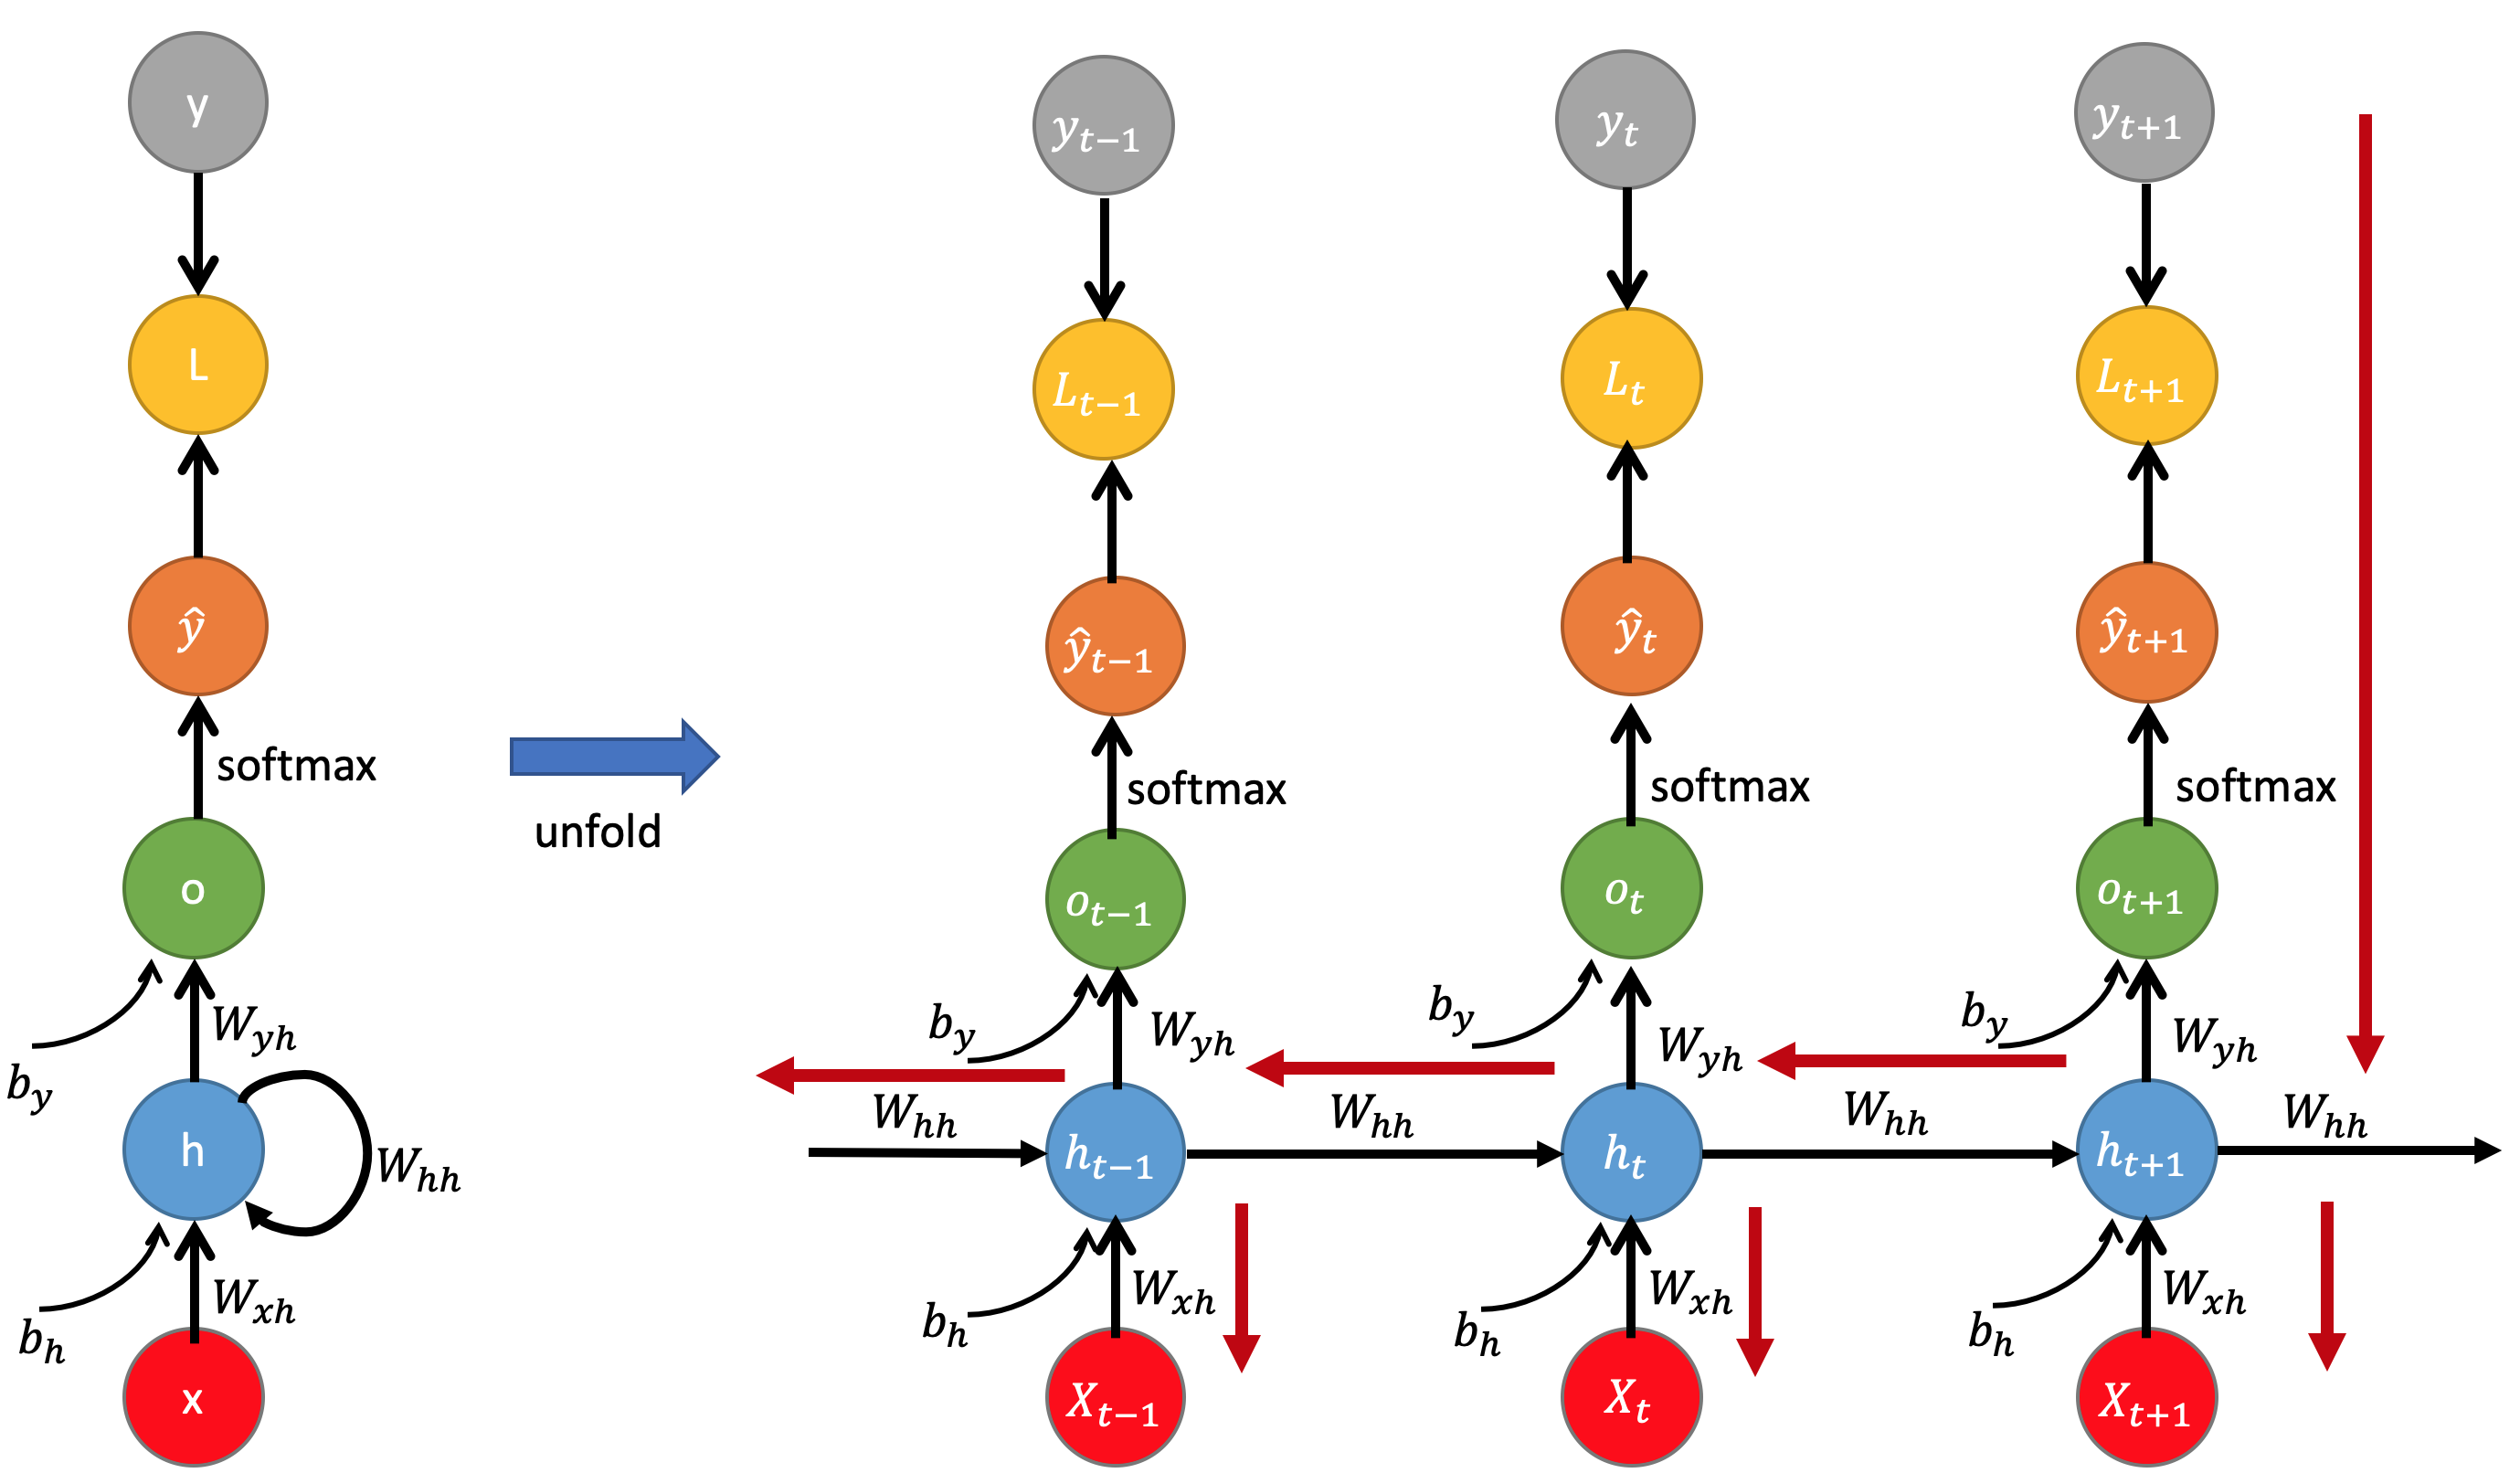
\includegraphics[width=0.8\textwidth]{figures/BPTT.png}
    \caption{BPTT 算法}
    \label{fig:s1}
\end{figure}

\begin{align*}
    h_t &= \Phi_h(X_t\cdot W_{xh}+h_{t−1}\cdot W_{hh}+b_h) \\
    o_t &= h_t\cdot W_{yh}+b_y \\
    \hat{y}_t &= \Phi_o(o_t) \\
    L &= \sum_{i=1}^T L_t \\
    L_t &= -[y_t\log\hat{y}_t+(1-y_t)\log(1-\hat{y}_t)]
\end{align*}

\begin{align*}
    \frac{\partial o_t}{\partial W_{yh}}
    &= h_t \\
    \frac{\partial o_t}{\partial h_t}
    &= W_{yh} \\
    \frac{\partial o_t}{\partial b_y}
    &= 1 \\
    \frac{\partial L_t}{\partial\hat{y}_t}
    &= -\frac{y_t}{\hat{y}_t}+\frac{1-y_t}{1-\hat{y}_t} \\
\end{align*}

\begin{align*}
    \Phi_o
    &= {\rm softmax} \\
    \frac{\partial\hat{y}_t}{\partial o_t}
    &= \hat{y}_t(1-\hat{y}_t) \\
    \frac{\partial L_t}{\partial o_t}
    &= \frac{\partial L_t}{\partial\hat{y}_t}\frac{\partial\hat{y}_t}{\partial o_t} \\
    &= \hat{y}_t-y_t \\
\end{align*}

\begin{align*}
    \frac{\partial L_t}{\partial b_y}
    &= \frac{\partial L_t}{\partial o_t}\frac{\partial o_t}{\partial b_y} \\
    &= \hat{y}_t-y_t \\
    \frac{\partial L_t}{\partial W_{yh}}
    &= \frac{\partial L_t}{\partial o_t}\frac{\partial o_t}{\partial W_{yh}} \\
    &= (\hat{y}_t-y_t)h_t \\
    \frac{\partial L_t}{\partial h_t}
    &= \frac{\partial L_t}{\partial o_t}\frac{\partial o_t}{\partial h_t} \\
    &= (\hat{y}_t-y_t)W_{yh} \\
    \frac{\partial L_{t+1}}{\partial W_{hh}}
    &= \frac{\partial L_{t+1}}{\partial h_{t+1}}\frac{\partial h_{t+1}}{\partial W_{hh}} \\
    &= \frac{\partial L_{t+1}}{\partial h_{t+1}}\frac{\partial h_{t+1}}{\partial h_t}\frac{\partial h_t}{\partial W_{hh}} \\
    &= \sum_{k=1}^{t+1}\frac{\partial L_{t+1}}{\partial h_{t+1}}\frac{\partial h_{t+1}}{\partial h_k}\frac{\partial h_k}{\partial W_{hh}} \\
    &= \sum_{k=1}^{t+1}\frac{\partial L_{t+1}}{\partial h_{t+1}}\left(\Pi_{j=k}^t\frac{\partial h_{j+1}}{\partial h_j}\right)\frac{\partial h_k}{\partial W_{hh}} \\
    \frac{\partial L_{t+1}}{\partial W_{xh}}
    &= \sum_{k=1}^{t+1}\frac{\partial L_{t+1}}{\partial h_{t+1}}\left(\Pi_{j=k}^t\frac{\partial h_{j+1}}{\partial h_j}\right)\frac{\partial h_k}{\partial W_{xh}} \\
\end{align*}

\begin{align*}
    \frac{\partial L}{\partial b_y}
    &= \sum_t^T\frac{\partial L_t}{\partial b_y} \\
    &= \sum_t^T\hat{y}_t-y_t \\
    \frac{\partial L}{\partial W_{yh}}
    &= \sum_t^T\frac{\partial L_t}{\partial W_{yh}} \\
    &= \sum_t^T(\hat{y}_t-y_t)h_t \\
    \frac{\partial L}{\partial W_{hh}}
    &= \sum_t^T\frac{\partial L_{t+1}}{\partial W_{hh}} \\
    &= \sum_t^T\sum_{k=1}^{t+1}\frac{\partial L_{t+1}}{\partial h_{t+1}}\left(\Pi_{j=k}^t\frac{\partial h_{j+1}}{\partial h_j}\right)\frac{\partial h_k}{\partial W_{hh}} \\
    \frac{\partial L}{\partial W_{xh}}
    &= \sum_t^T\frac{\partial L_{t+1}}{\partial W_{xh}} \\
    &= \sum_t^T\sum_{k=1}^{t+1}\frac{\partial L_{t+1}}{\partial h_{t+1}}\left(\Pi_{j=k}^t\frac{\partial h_{j+1}}{\partial h_j}\right)\frac{\partial h_k}{\partial W_{xh}} \\
\end{align*}

\section{复现文献}

\begin{itemize}
    \item \href{https://www.frontiersin.org/articles/10.3389/fnins.2018.00331/full}{Spatio-temporal backpropagation for training high-performance spiking neural networks}
\end{itemize}

% \begin{figure}[hb]
%     \centering
%     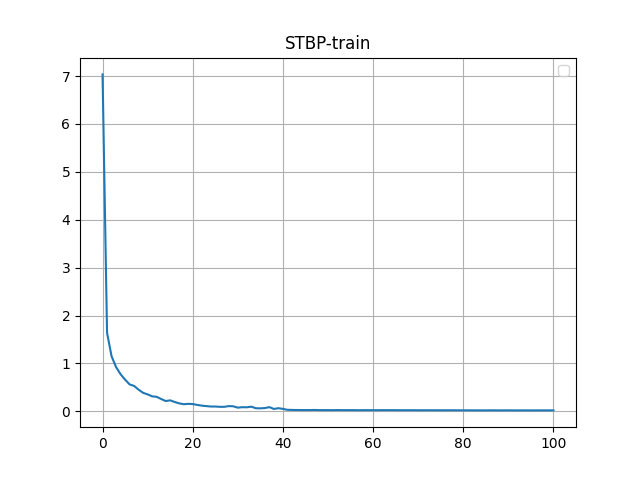
\includegraphics[width=0.8\textwidth]{figures/STBP-train.png}
%     \label{fig:s1}
% \end{figure}

% \begin{figure}[hb]
%     \centering
%     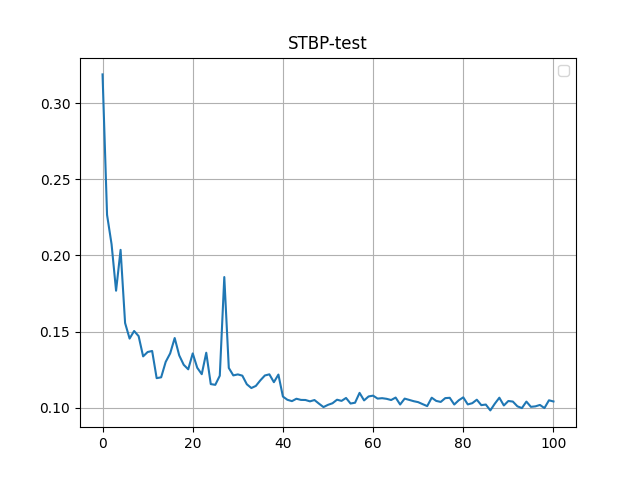
\includegraphics[width=0.8\textwidth]{figures/STBP-test.png}
%     \label{fig:s1}
% \end{figure}

\begin{figure}[hb]
    \centering
    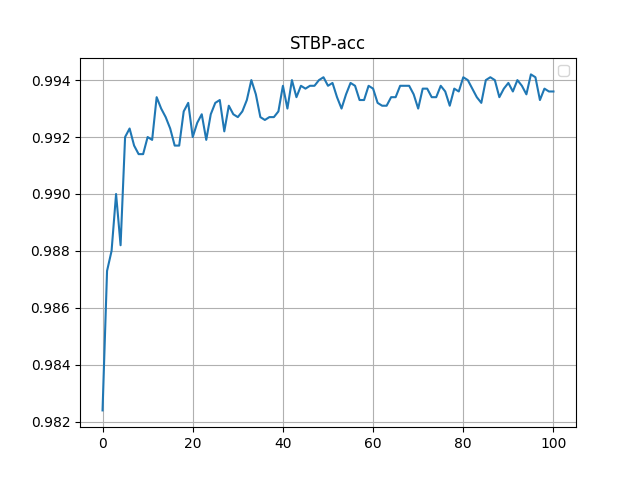
\includegraphics[width=0.8\textwidth]{figures/STBP-acc.png}
    \label{fig:s1}
\end{figure}

\section{阅读文献}

\begin{itemize}
    \item \href{https://arxiv.org/abs/2005.02183}{Comparing SNNs and RNNs on Neuromorphic Vision Datasets: Similarities and Differences}
    \item \href{https://arxiv.org/abs/1811.10766}{Synaptic Plasticity Dynamics for Deep Continuous Local Learning}
    \item \href{http://ir.hit.edu.cn/~jguo/docs/notes/bptt.pdf}{BackPropagation Through Time}
\end{itemize}

\section{其它}

参加 \href{https://box.nju.edu.cn/f/c970af185163433d9a38/}{2023开源软件论坛} 暨 GFWJWG 第二次会议.

\end{document}
